\chapter{Stationary states and stability}\label{Stationary states and stability}
%\begin{aquote}{Wild Thing. J. Bazell 2013.}
%\textit{In metric, one milliliter of water occupies one cubic centimeter, weighs one gram, and requires one calorie of energy to heat up by one degree centigrade — which is 1 percent of the difference between its freezing point and its boiling point. An amount of hydrogen weighing the same amount has exactly one mole of atoms in it. Whereas in the [imperial] system, the answer to "How much energy does it take to boil a room-temperature gallon of water?" is ``Go fuck yourself'', because you can't directly relate any of those quantities.}
%\end{aquote}
Now that we are able to model and simplify a physical system, we want to predict what the equations will do without having to simulate the system each time. Specifically, we are not interested in the transient initial behaviour of the equations, we want to understand what the trajectories will like far into the future. In one dimension we have proven that the equations must either monotonically increase, decrease, or tend to a fixed value. In two-dimensions we have the additional complications of persistent oscillatory dynamics. In higher dimensions we have the further option of chaotic systems, which are outside the scope of this course. However, even by restricting ourselves to one and two dimensions, how do we know what will happen? To enable us to generate these insights we first need two important definitions.
\begin{defin}
A state, $\bm{u}_s$, is a \textbf{steady state} or \textbf{stationary state} of the ODE system
\bb
\dot{\bm{u}}=\bm{F}(\bm{u})
\ee
if is satisfies $\bm{F}(\bm{u}_s)=0$.
\end{defin}
This definition simply states that if the ODE system ever reaches $\bm{u}_s$ then the system will not evolve further because all of the dynamics are in equilibrium. This is a useful concept, but currently incomplete.

For example, you can (theoretically) stand a pencil on its tip and it would remain stationary, if it were not perturbed \see{Pencil_stationary_state}. Hence, this is a stationary state orientation of the pencil. However, it would require only a very small perturbation to cause the coin to fall over and, thus, transition from the state of being on its point to being on its side \see{Pencil_stationary_state}. Given a large enough perturbation (\ie picking the pencil up) you could reset the pencil to the previous state of standing on its point. However, it requires a larger perturbation to reset the pencil than it does to knock it over and, so, we see that although these state are both stationary states they are somehow fundamentally different. This difference comes down to the intuitive concept of `stability'.
\begin{figure}[!!!h!!!tb]
\centering
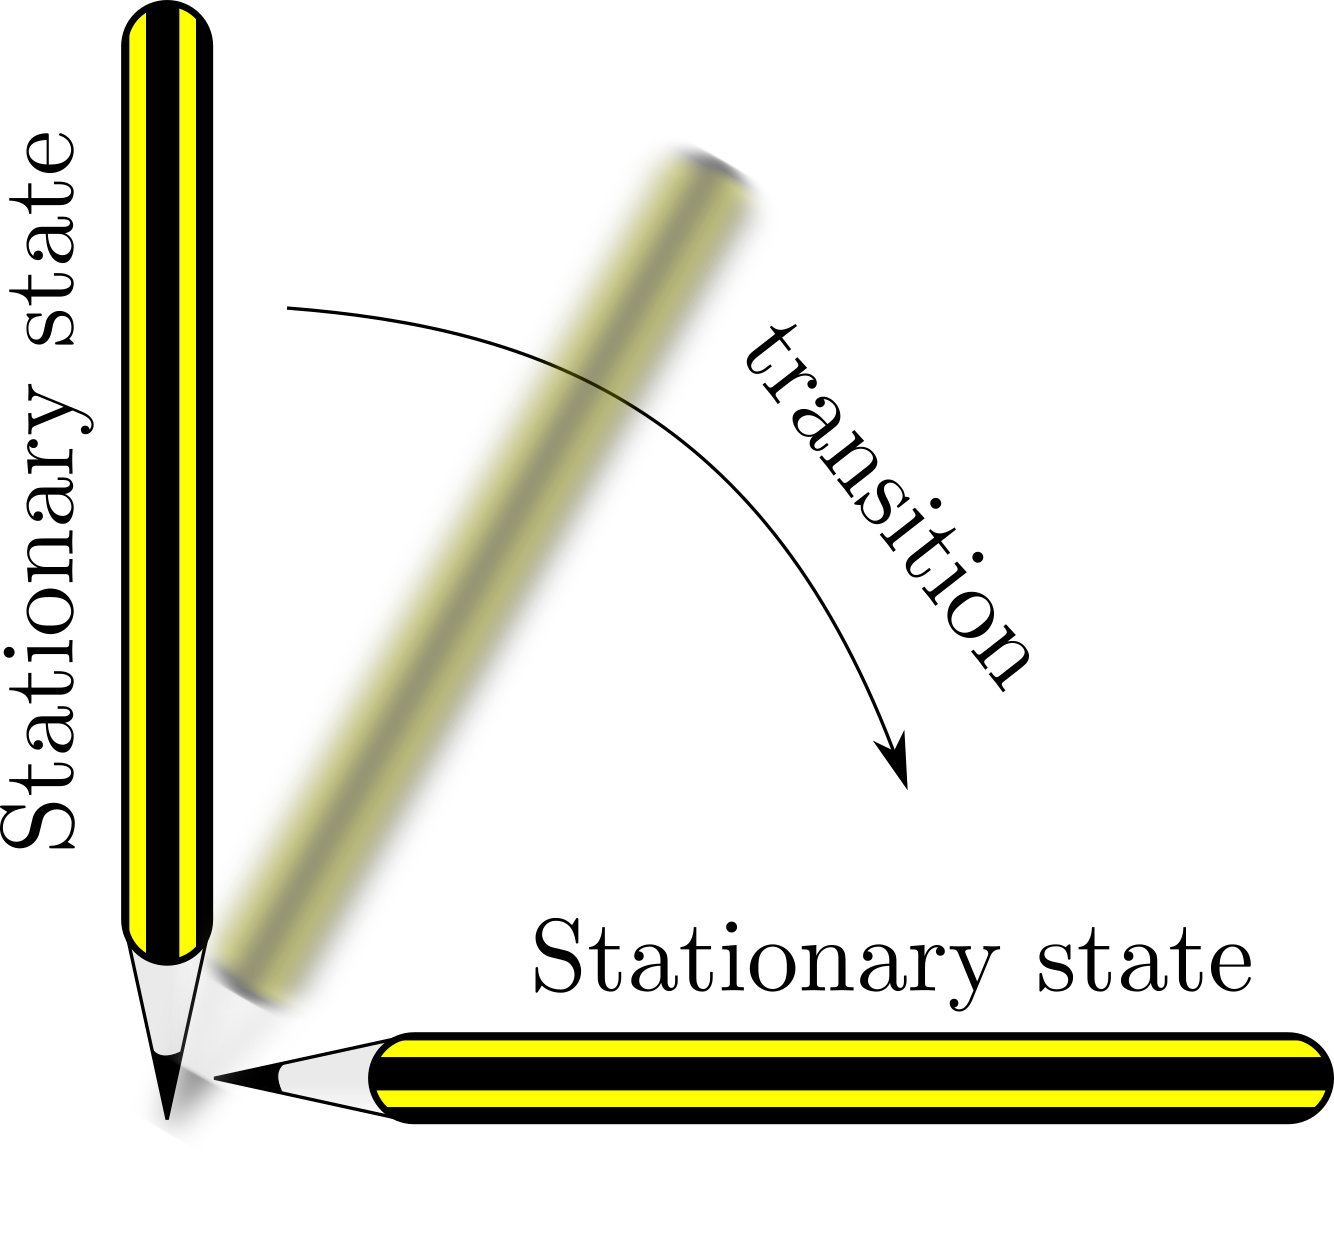
\includegraphics[width=\ttp]{../Pictures/Pencil_stationary_state.png}
\caption{\label{Pencil_stationary_state} Stationary states of a pencil.}
\end{figure}

\begin{defin}
A steady state, $\bm{u}_s$, of the ODE system
\bb
\dot{\bm{u}}=\bm{F}(\bm{u})
\ee
is \textbf{stable} if for all $\epsilon >0$, there exists a $\delta > 0$ and a $t_0>0$ such that whenever $|\bm{u}(t)-\bm{u}_s|< \delta$ then $|\bm{u}(t)-\bm{u}_s|<\epsilon$ for all $t \ge t_0$. Otherwise the steady state is unstable
\end{defin}
Simply put, this means that a state, $\bm{u}_s$, is stable if whenever a solution $\bm{u}(t)$ comes close enough to it then the solution tends to the state \ie $\bm{u}(t)\rightarrow\bm{u}_s$. In the example of the pencil, both the vertical and horizontal orientations of the pencil are stationary state. However, only the horizontal orientation is stable.

\begin{example}[frametitle=Balls on surfaces]
Consider \fig{Stationary_stability}, using your intuition, state which of the balls are stationary and which are stable, assuming that the surface that they are moving on has a small amount of friction.
\COL{
\begin{enumerate}[label=(\alph*)]
\item Stationary and stable. This ball is `\textit{globally}' stable, namely, no matter how big a perturbation is given, the ball will always end up at the bottom of the well. Note, that if the surface had no friction the ball wall oscillate to and fro forever.
\item Stationary and unstable. The surface is only flat at one point, thus, any perturbation will cause the ball to slide away from the central point.
\item Non-stationary and, thus, cannot be categorised as stable, or unstable. The surface is not locally flat anywhere, so the ball simply keeps moving.
\item Stationary and stable. However, this ball is only `\textit{locally}' stable (compare with (a)). A big enough perturbation will cause the ball to exist the stability region and not return back to the stationary state.
\item Stationary and unstable. This case is similar to (b).
\end{enumerate}
}
\end{example}
\begin{figure}[!!!h!!!tb]
\centering
\includegraphics[width=\tp]{../Pictures/Stationary_stability.png}
\caption{\label{Stationary_stability} Which balls are stationary and stable?}
\end{figure}

Moving beyond the case of categorising drawings let us consider the specific mathematical example of the logistic equation.
\begin{example}[frametitle=Stationary states and stability of the logistic equation\label{Logistic_stability_example}]
The non-dimensionalised logistic equation is (as we have seen before)
\bb
\dot{u}=u(1-u).\label{Logistic_stability}
\ee
\COL{Firstly, we calculate the steady states by setting $\dot{u}=0$. Trivially, we can see that the steady }\COL{are $u=0$ and $1$. Later, we will see how to derive the stability of a general system analytically. Here, we will develop our curve sketching techniques, specifically,  plot \eqn{Logistic_stability} in the $(u,\dot{u})$ coordinate plane \see{Logistic_phase_plane}.

In the top half plane $\dot{u}>0$ and, thus, $u$ increases over time. Equally, in the bottom half plane $\dot{u}<0$ and $u$ decreases over time. Drawing arrows on \fig{Logistic_phase_plane} to illustrate these facts demonstrates that $u=0$ is unstable as trajectories diverge away from it, whilst $u=1$ is stable as trajectories tend to this state. The insights gained from \fig{Logistic_phase_plane} are confirmed in \fig{Logistic_multi_IC}, where, from simulating multiple initial conditions, we see that any small (positive) perturbation away from zero causes the solution to converge to $u=1$, eventually. Equally, any initial condition $u>1$ decreases monotonically towards $u=1$, too.}
\end{example}
\begin{figure}[!!!h!!!tb]
\centering
\subfigure[\label{Logistic_phase_plane}]{\includegraphics[width=\ttp]{../Pictures/Logistic_stability.png}}
\subfigure[\label{Logistic_multi_IC}]{\includegraphics[width=\ttp]{../Pictures/Logistic_multi_IC.png}}
\caption{ \label{Logistic_figure}Illustrating the stationary states and stability characteristics of the logistic \eqn{Logistic_stability}. (a) A plot of the curve in $(u,\dot{u})$ coordinates. (b) Multiple simulations of \eqn{Logistic_stability} with different initial conditions, $u_0$, noted in the legend.}
\end{figure}
As we saw in example \ref{Logistic_stability_example}, when working with a single dependent variable, $u$, all of the stationary and stability information can be gained from plotting the `phase plane', \ie the $(u,\dot{u})$ coordinate system. Specifically, the stationary states are given where the curve crosses the `$x$-axis' (\ie $\dot{u}=0$) and the stability of the states can be given by considering where the the system is increasing or decreasing in the vicinity of the stationary point (\ie the sign of $\dot{u}$).

However, drawings can be misleading and may not be possible if the function on the right-hand side of the differential equation is too complicated. Equally, drawing the curve will not work if the system has more than one variable. Thus, we need an analytical method to characterise the stability of a system, which can be generalised to higher order systems.

\section{Linear stability}
The crux of this method is to consider the dynamics of an ODE system near its stationary points. To do this we substitute a solution into the equations that is a perturbation about the steady state. Using Taylor series we expand the system in terms of the perturbation and keep only the linear terms as we are assuming that the perturbation is small. Since the system is now linear we can solve the approximate equations completely and, thus, they will tell us what dynamics to expect close to the steady states.
\begin{thm}\label{Stability_theorem}
Suppose $u_s$ is a steady state of the one dimensional ODE,
\bb
\dot{u}=F(u),\label{General_ODE}
\ee
then $u_s$ is linearly stable if $\rd F(u_s)/\rd u<0$ and linearly unstable if $\rd F(u_s)/\rd u>0$.
\end{thm}
\begin{proof}
\COL{Consider a solution of the form $u(t)=u_s+\epsilon(t)$, where $|\epsilon(0)| \ll 1$. Substituting the perturbed solution into \eqn{General_ODE}, we find that
\bb
\dot{\epsilon}=F(u_s+\epsilon).
\ee
We now use Taylor's theorem on the right-hand side to derive the approximation
\bb
F(u_s+\epsilon)\approx F(u_s)+\epsilon \frac{\rd F}{\rd u}(u_s)+\frac{\epsilon^2}{2} \frac{\rd^2 F}{\rd u^2}(u_s)+\dots.
\ee
Ignoring all terms except the linear order in $\epsilon$ we conclude that initially
\bb
\dot{\epsilon}\approx F(u_s)+\epsilon \frac{\rd F}{\rd u}(u_s).
\ee
By assumption $u_s$ is a stationary point and, thus, by definition, $F(u_s)=0$. Hence, approximately,
\bb
\dot{\epsilon}=\epsilon \frac{\rd F}{\rd u}(u_s).\label{Linear_eqn}
\ee
Equation \eqref{Linear_eqn} is trivially solvable since $\rd F(u_s)/\rd u$ is a constant,
\bb
\epsilon(t)=\epsilon(0)\exp\l t\frac{\rd F}{\rd u}(u_s)\r.
\ee
The exponential solution form tells us that if $\rd F(u_s)/\rd u<0$ then $\epsilon(t)\rightarrow 0$ as $t\rightarrow \infty$. This means that our small perturbation dies out over time and the solution $u(t)\rightarrow u_s$ as $t\rightarrow \infty$. In other words $u_s$ is stable because solutions that are slightly perturbed away from $u_s$ tend to evolve back to $u_s$.

Oppositely, if $\rd F(u_s)/\rd u>0$ then $\epsilon(t)\rightarrow \infty$ as $t\rightarrow \infty$. Thus, the solution diverges away from $u_s$ meaning that $u_s$ is unstable.}
\end{proof}
We make a number of remarks about the theorem's statement and proof:
\COL{
\begin{itemize}
\item the theorem makes no claim about the solutions properties in the case that the first derivative $\rd F(u_s)/\rd u=0$. In this specific case we would have to go to higher order in the Taylor expansion.
\item the proof does not specify the size of $\epsilon$, thus, the steady state may be globally stable, in that all trajectories tend to $u_s$. However, the proof only assures us of the local stability.
\item in the case that $u_s$ is unstable we cannot conclude what happens to the trajectory. Specifically, although $\epsilon$ will grow exponentially, this simply means that our approximation of small $\epsilon$ is no longer valid. Indeed, a trajectory near an unstable point may grow without bound or, simply tend to one of the other stationary states in the system that are stable.
\end{itemize}
}
\begin{example}[frametitle=Linearising around multiple steady states]\label{Multi_stable_example}
Consider the following equation, which can be used to model harvesting, with constant effort, $E>0$, of a population, $u$,
\bb
\dot{u}=f(u)=\underbrace{\frac{2u^2}{u^2+1}}_{\textrm{Population growth with saturating rate}}-\underbrace{Eu}_{\textrm{Constant harvesting effort}}.\label{Multi_stable_eqn}
\ee
\COL{The steady states are solutions to
\bb
0=f(u)=\frac{2u^2}{u^2+1}-Eu,\label{St_st_1}
\ee
and, so,
\bb
u_s=0,\frac{1\pm\sqrt{1-E^2}}{E}.\label{us_1}
\ee
Name these states $u_0$, $u_-$ and $u_+$ in the obvious way. Since we are dealing with a real system we must ensure that the steady states are also real. Namely, the states $u_\pm$ only exist when $0<E\leq 1$; if $E>1$ only $u_0$ exists. Finally, $u_\pm>0$ for all values of $0<E\leq 1$.


Now let us consider the derivative of $f$ in order to prescribe stability
\begin{align}
f'(u)&=\frac{4u(u^2+1)-4u^3}{(u^2+1)^2}-E\\
&=\frac{4u}{(u^2+1)^2}-E.
\end{align}
We now check each steady state separately. Since
\bb
f'(0)=-E<0
\ee
we immediately conclude that $u_0$ is a linearly stable stationary state. Similarly,
\bb
f'(u_+)=\frac{E \l (E^2-2)\sqrt{1-E^2}+2(E^2-1) \r }{ \l 1+\sqrt{1-E^2} \r^2}.
\ee
Thus, we have to contend with showing whether $f'(u_+)$ is positive, or negative, and how that depends on $E$. Firstly, we note that $\l 1+\sqrt{-E^2+1} \r^2$ is always positive, so it is only the numerator that could change sign. Equally, by definition $u_+$ only exists if $0<E<1$, thus we can also eliminate the factor of $E$ at the front of the equation. Hence, we reduce the stability problem to determining the sign of
\bb
(E^2-2)\sqrt{1-E^2}+2\l E^2-1\r.
\ee}
\COL{Since $0<E<1$ then both $(E^2-2)$ and $(E^2-1)$ are negative, hence $f'(u_+)<0$, and, so, $u_+$ is stable. Similarly
\bb
f'(u_-)=\frac { \l (2-E^2)\sqrt {1-E^2}+2(E^2-1) \r E}{ \l -1+\sqrt {E^2-1} \r ^{2}}.
\ee
Unfortunately, this case is not so clear cut, because $\l 2-E^2\r>0$, but $(E^2-1)<0$. We could continue investigating the properties of the curve
\bb
(2-E^2)\sqrt {1-E^2}+2(E^2-1),
\ee
but this is not so easy. Instead, we consider $f'(u_-)$ without substituting in the value of \eqn{us_1}. Further, we note that by rearranging \eqn{St_st_1} $u_-$ is a solution of
\bb
0=2u_--E(u_-^2+1)\implies \frac{2u_-}{E}=(u_-^2+1).
\ee
Thus,
\begin{align}
f'(u_-)&=\frac{4u_-}{(u_-^2+1)^2}-E,\\
&=\frac{E^2}{u_-}-E,\\
&=\frac{E}{u_-}\l E-u_-\r.
\end{align}
As mentioned above $u_->0$, thus, the sign of $f'(u_-)$ depends solely on the sign of
\begin{align}
E-u_-&=E-\frac{1-\sqrt{1-E^2}}{E},\\
&=\frac{-(1-E^2)+\sqrt{1-E^2}}{E},\\
&=\frac{-a+\sqrt{a}}{E},
\end{align}
where, in the last line we have defined $a=1-E^2$. Now, since $0<E<1$ then $0<a<1$, and, so, $a<\sqrt{a}$, hence $E-u_->0$, resulting in the discovery that $f'(u_-)>0$ for all $E$, meaning that $u_-$ is unstable.

In summary $u_0$ is always stable. The steady states $u_\pm$ only exist when $0<E<1$ and whenever they do exist $u_+$ is linearly stable, whilst $u_-$ is unstable.

Of course, we could have seen this much easier if we had simply plotted $f(u)$ as shown in \fig{Multi_stable_figure}. \fig{Multi_stable_figure} also provides us with the information of which initial conditions will go to which steady state. Specifically, in the case that $0<E<1$, if $u(0)<u_-$ then the population will tend to zero, whilst if $u(0)>u_-$ the population will tend to $u_+$. Equally, we see that in the case when $E>1$ all populations tend to zero.

Although, the graphical method is easier to use in this case, we may have missed certain cases if we had just drawn one graph. Equally, we have the explicit existence bounds on $u_\pm$. Finally, the derivative method presented in Theorem \ref{Stability_theorem} is more easily extended to higher dimensions, as we will see later.

The interpretation of these results provide serious implications on the viability of a harvested population. Namely, if we are greedy and harvest too much of the population ($E>1$) then }\COL{the population will go extinct. Moreover, even if $0<E<1$ and, so, sustainable harvesting is }\COL{possible, we still have to ensure that the population is large enough to take the impact. Namely, since $u_0$ is stable, then a small population will die out, no matter how small the harvesting effort is. Critically, only in the no harvesting case $E=0$ are we guaranteed to have a surviving population.}
\end{example}
\begin{figure}[!!!h!!!tb]
\centering
\subfigure[\label{Multi_stable_phase_plane_E9} $E=0.9$]{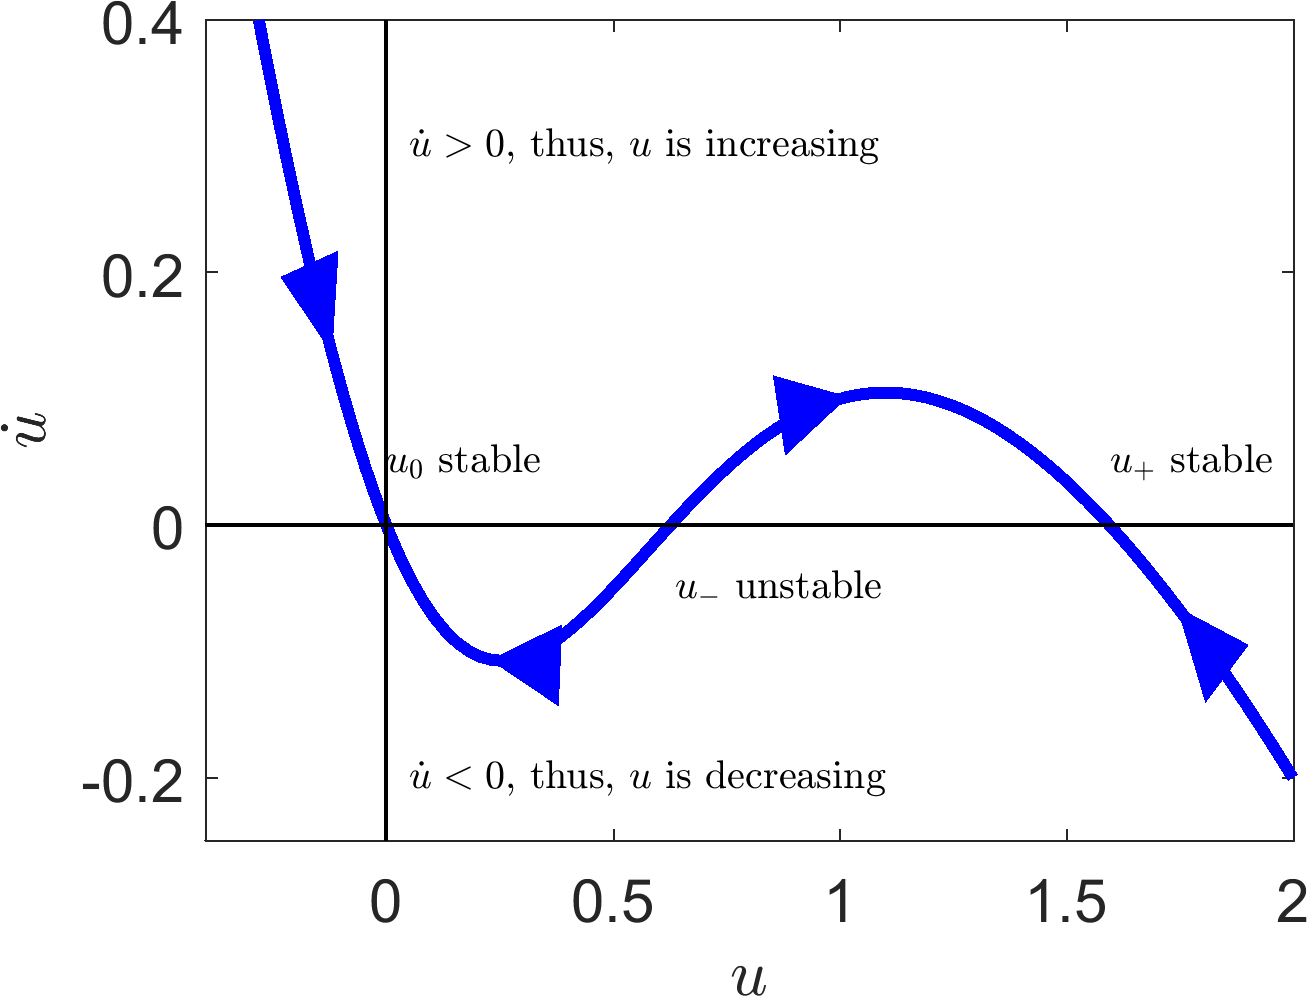
\includegraphics[width=\ttp]{../Pictures/Multi_stable_stability_E9.png}}
\subfigure[\label{Multi_stable_multi_IC_E9} $E=0.9$]{\includegraphics[width=\ttp]{../Pictures/Multi_stable_multi_IC_9.png}}
\subfigure[\label{Multi_stable_phase_plane_E11} $E=1.1$]{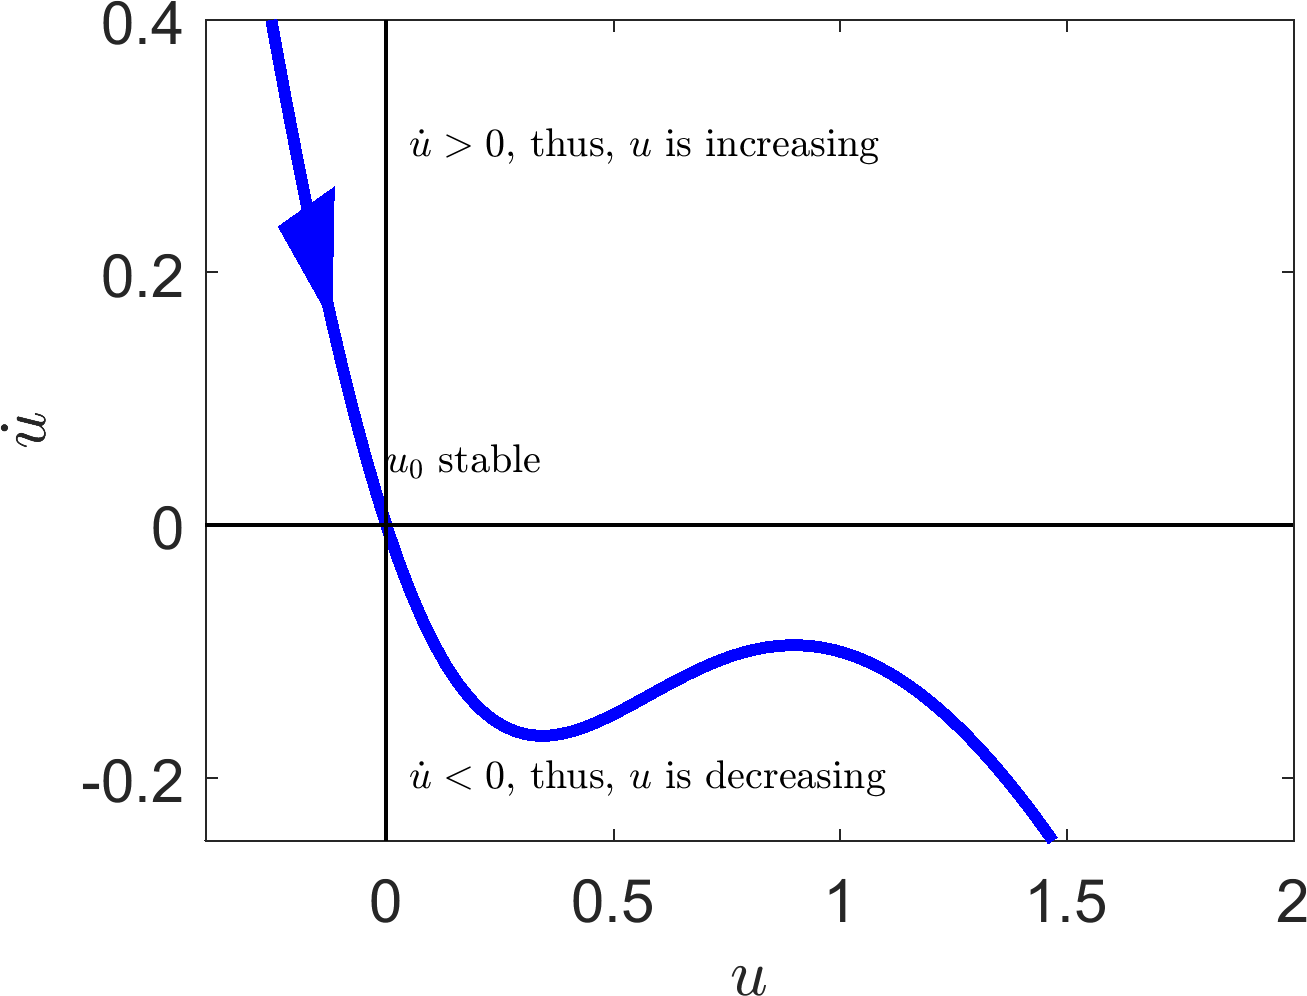
\includegraphics[width=\ttp]{../Pictures/Multi_stable_stability_E11.png}}
\subfigure[\label{Multi_stable_multi_IC_E11} $E=1.1$]{\includegraphics[width=\ttp]{../Pictures/Multi_stable_multi_IC_11.png}}
\caption{ \label{Multi_stable_figure}Illustrating the stationary states and stability characteristics of \eqn{Multi_stable_eqn}. Top row: case when $E=0.9$ and three steady states exist. (a) A plot of the curve in $(u,\dot{u})$ coordinates. (b) Multiple simulations of \eqn{Multi_stable_eqn} with different initial conditions, $u_0$, noted in the legend.  Bottom row: case when $E=1.1$ and only $u_0=0$ is a stationary state. (a) A plot of the curve in $(u,\dot{u})$ coordinates. (b) Multiple simulations of \eqn{Multi_stable_eqn} with different initial conditions, $u_0$, noted in the legend.}
\end{figure}

\section{Bifurcations and hysteresis}\label{Hysteresis}
As seen in example \ref{Multi_stable_example} the existence and stability of steady states can depend on model parameters, here $E$.
\begin{defin}
A \textbf{bifurcation point} of a system is a parameter value at which the characteristics of the steady states change. This can be either in number of steady states, or their stability.
\end{defin}
In example \ref{Multi_stable_example}, $E=1$ is a bifurcation point of the system.

The amount of information gained in example \ref{Multi_stable_example} can be quite overwhelming. Thus, we use a bifurcation diagram to illustrate the complexity in a simple way. Specifically, \fig{Hysteresis_figure} shows \eqn{us_1} as a function of $E$ and captures the following features:
\begin{itemize}
\item $u_0$ always exists;
\item $u_\pm$ exists whenever $E<1$;
\item $u_0$ and $u_+$ are stable when they exist;
\item $u_-$ is always unstable when it exists.
\end{itemize}

\fig{Hysteresis_figure} can also be used to tell us what happens in the case when we think about varying $E$ and how it can have unexpected impacts on the system. Consider the case where we are happily fishing in a lake, which can be modelled by \eqn{Multi_stable_eqn}, such that $E=0.7$ and, so the level of fish in the lake is stable at around $u_+(0.7)\approx 2$ (taken from \fig{Hysteresis_figure}\footnote{We are assuming that the system is non-dimensionalised, so I am not saying this is two fish, or two tons, just a measure of two times some scale.}).

Suppose we become greedy and increase our effort, thus pushing $E$ to 1.1. The population begins to die out rapidly, due to over fishing. Critically, we notice the huge reduction in population size and reduce our effort to the previous stable case, $E=0$. Unfortunately, we have left it too late and the population has reduced past $u_-(0.7)$, thus, even though a fish population still exists and our harvesting rate $E<1$, the population will still die. This is an example of hysteresis.
\begin{figure}[!!!h!!!tb]
\centering
\includegraphics[width=0.7\textwidth]{../Pictures/Hysteresis.png}
\caption{ \label{Hysteresis_figure}Bifurcation plot of \eqn{Multi_stable_eqn}. The dependence of the existence and stability of $u_0$, $u_-$ and $u_+$ on $E$ is plotted. The $u_-$ is dashed to illustrate that the steady states are always unstable, whilst $u_0$ and $u_+$ are stable wherever they exist. However, the steady states, $u_\pm$, disappear for $E>1$.}
\end{figure}
\begin{defin}
A system exhibits \textbf{hysteresis} if, when a parameter of the system is altered and subsequently returned to the initial value, the system does not return to its original state.
\end{defin}

Example \ref{Multi_stable_example} and \fig{Hysteresis_figure} demonstrate a simple way showing a system exhibits hysteresis. Specifically, you should:
\begin{enumerate}
\item derive the steady states and their dependence on any given parameters;
\item derive the stability of the  steady states and their dependence on any given parameters;
\item note any bifurcation points of the parameters;
\item define and illustrate the characteristics of the system before and after the bifurcation point;
\item consider the system before the bifurcation point;\label{biff_1}
\item identify what happens to the system as the bifurcation increases passes its bifurcation point;
\item identify what happens to the system as the bifurcation is reduced to its initial value;\label{biff_2}
\item if the system state in point \ref{biff_1} is the same as \ref{biff_2} then the system does not exhibit hysteresis. Otherwise hysteresis is present in the system.
\end{enumerate}

%\begin{example}[frametitle=Failure]
%As mentioned not all balances are valid, which is what we will seen in this example. %Consider the following ODE system
%\begin{align}
%  \tikzmark{a}\dot{u}=k_0\tikzmark{b}+k_1\tikzmark{c}u-k_2uv, \quad u(0)=u_0,\label{Non-dim_9}\\
% \nonumber \\
%    \tikzmark{e}\dot{v}=k_3\tikzmark{f}+k_4\tikzmark{g}v-k_2uv, \quad v(0)=v_0.\label{Non-dim_10}
%\tikz[overlay,remember picture]
%{\draw[square arrow1] (a.south) to (b.south);}
%\tikz[overlay,remember picture]
%{\draw[square arrow1] (b.south) to (c.south);}
%\tikz[overlay,remember picture]
%{\draw[square arrow1] (e.south) to (g.south);}
%%\end{align}
%There are three variables $u$, $v$ and $t$ and so we need three balances. The chosen balances are illustrated on the equations using arrows. Extracting information from the balances we find that
%\bb
%\frac{[u]}{[t]}=k_0=k_1[u], \quad \frac{[v]}{[t]}=k_4[v].
%\ee
%From this point we quickly discover that
%\bb
%[t]=\frac{1}{k_1} \textrm{ and } [t]=\frac{1}{k_4}.
%\ee
%Since, generally, $k_1\neq k_4$ we cannot satisfy both balances, thus, we must consider a different non-dimensionalisation.
%
%One possible valid non-dimensionalisation is
%\begin{align}
%  \tikzmark{a}\dot{u}=k_0\tikzmark{b}+k_1\tikzmark{c}u-k_2uv, \quad u(0)=u_0,\nonumber\\
% \nonumber \\
%    \tikzmark{e}\dot{v}=k_3\tikzmark{f}+k_4\tikzmark{g}v-k_2uv, \quad v(0)=v_0.\nonumber
%\tikz[overlay,remember picture]
%{\draw[square arrow1] (a.south) to (b.south);}
%\tikz[overlay,remember picture]
%{\draw[square arrow1] (b.south) to (c.south);}
%\tikz[overlay,remember picture]
%{\draw[square arrow1] (e.south) to (f.south);}
%\end{align}
%See your problem sheets for details.
%\end{example}


%\begin{figure}[!!!h!!!tb]
%\centering
%\subfigure[\label{IC_0.1}]{\includegraphics[width=\ttp]{../Pictures/Comparing_pendulums_IC_1.png}}
%\subfigure[\label{IC_1}]{\includegraphics[width=\ttp]{../Pictures/Comparing_pendulums_IC_10.png}}
%\caption{\label{Different_ICs}Comparing \eqns{Spring_eqn}{Bob_eqn} with initial conditions (a) $y=0=\theta$ and (b) $y=1=\theta$. Parameter values $r=g=k=m=1$.}
%\end{figure}
%
%
%\begin{example}[frametitle=Zombies]\label{Zombies}
%Humans, $H$ and zombies, $Z$ interact through the following three interactions \see{Zombie_picture}]:
%\end{example}
%\begin{figure}[!!!h!!!tb]
%\centering
%\includegraphics[width=\tp]{../Pictures/Zombies.png}
%\caption{\label{Zombie_picture} Possible outcomes of human-zombie interactions.}
%\end{figure}

\section{Check list}
By the end of this chapter you should be able to:
\begin{todolist}
\item derive the steady states of a system;
\item categorise the stability of the steady states using graphical means;
\item prove that the stability of a steady state depends on the sign of the first derivative (with respect the system variable) evaluated at the steady state;
\item analytically specify the parameter dependencies of the steady states and stability criteria;
\item identify bifurcation points;
\item plot the steady state curves in a bifurcation diagram;
\item identify whether a system could exhibit hysteresis. 
\end{todolist}




